% Carrusel del perfil del proyecto (Expo Ingenierías, Anexo 6): 3 imágenes que se explican solas.
% Página 1 = fondo del GIF (la animación de los edificios se monta en el hueco de la derecha).
\documentclass{article}
\usepackage[paperwidth=40cm,paperheight=22.5cm,margin=0cm]{geometry}
\usepackage{fontspec}
\usepackage[spanish]{babel}
\usepackage{xcolor,graphicx,tikz}
\usetikzlibrary{calc}
\pagestyle{empty}
\setmainfont{SourceSans3}[Extension=.otf, UprightFont=*-Regular, BoldFont=*-Bold, ItalicFont=*-RegularIt, FontFace={sb}{n}{*-Semibold}]
\newfontfamily\serif{SourceSerif4}[Extension=.otf, UprightFont=*-Regular, BoldFont=*-Bold, ItalicFont=*-RegularIt]
\newcommand\sbf{\fontseries{sb}\selectfont}
\hyphenpenalty=10000 \exhyphenpenalty=10000
\definecolor{tinta}{HTML}{1D2440}\definecolor{noche}{HTML}{0F1533}\definecolor{gris}{HTML}{6B6F80}\definecolor{papel}{HTML}{FBF8F2}
\definecolor{hogar}{HTML}{C8553D}\definecolor{escuela}{HTML}{2E6FA7}\definecolor{alto}{HTML}{3C3570}\definecolor{oro}{HTML}{E9B44C}\definecolor{crema}{HTML}{F3EEE3}
\newcommand\pie[1]{\node[anchor=south west, text=#1, font=\fontsize{14}{17}\selectfont] at ([xshift=1.6cm, yshift=0.8cm]current page.south west)
  {Desigualdad en el acceso a la lectura en la infancia · Datos: INEGI, MOLEC 2019–2024 · Tecnológico de Monterrey · Expo Ingenierías};}
\newcommand\paso[2]{\node[anchor=north west, text=oro, font=\sbf\fontsize{17}{20}\selectfont] at ([xshift=1.6cm, yshift=-1.3cm]current page.north west) {#1 \textcolor{#2}{/ 3}};}
\begin{document}
% =============================================================== 1 · el problema y el hallazgo (fondo del GIF)
\pagecolor{noche}
\begin{tikzpicture}[remember picture, overlay]
  \paso{1}{white!50!noche}
  \node[anchor=north west, text width=14.6cm, align=left, text=white, font=\serif\bfseries\fontsize{38}{44}\selectfont] at ([xshift=1.6cm, yshift=-2.5cm]current page.north west)
    {¿Leer de adulto depende de cómo creciste?};
  \node[anchor=north west, text width=14.6cm, align=left, text=white!88!noche, font=\fontsize{20}{27}\selectfont] at ([xshift=1.6cm, yshift=-8.3cm]current page.north west)
    {En México, solo \textcolor{oro}{\textbf{4 de cada 10}} adultos que saben leer leyeron al menos un libro en el último año.\par\vspace{0.45cm}
     Analizamos a \textbf{11,685 adultos} de la encuesta del INEGI y los separamos según los estímulos de lectura que tuvieron \textbf{en su casa} cuando eran niños:\par\vspace{0.3cm}
     {\fontsize{19}{25}\selectfont\color{oro}\textbullet\ \color{white!88!noche}había libros en casa \ \color{oro}\textbullet\ \color{white!88!noche}le leían\\
      \color{oro}\textbullet\ \color{white!88!noche}veía leer a sus padres\ \color{oro}\textbullet\ \color{white!88!noche}lo llevaban a bibliotecas}};
  % hueco de la animación: 1080 x 608 px desde (816, 150) px  → en cm: x 17.0, y 3.125, ancho 22.5, alto 12.66
  \draw[white!25!noche, line width=2pt, rounded corners=6pt] ([xshift=16.95cm, yshift=-3.075cm]current page.north west) rectangle ++(22.6, -12.76);
  \node[anchor=north west, text width=22.4cm, align=left, text=white, font=\fontsize{22}{29}\selectfont] at ([xshift=17.0cm, yshift=-16.4cm]current page.north west)
    {De quienes tuvieron \textcolor{oro}{\textbf{mucho acceso}} a la lectura en casa (3 o 4 estímulos), leyó al menos un libro el \textcolor{oro}{\textbf{59.7\,\%}}; de quienes tuvieron poco (0 o 1), solo el \textbf{28.1\,\%}: aproximadamente la mitad.};
  \node[anchor=north west, text=white!55!noche, font=\fontsize{15}{18}\selectfont] at ([xshift=17.0cm, yshift=-19.5cm]current page.north west)
    {Cada ventana encendida representa a los lectores de cada grupo · asociación, no causalidad};
  \pie{white!55!noche}
\end{tikzpicture}
\newpage
% =============================================================== 2 · casa o escuela
\pagecolor{papel}
\begin{tikzpicture}[remember picture, overlay]
  \fill[tinta] (current page.north west) rectangle ([yshift=-5.6cm]current page.north east);
  \paso{2}{white!50!tinta}
  \node[anchor=north west, text=white, font=\serif\bfseries\fontsize{38}{44}\selectfont] at ([xshift=1.6cm, yshift=-2.4cm]current page.north west)
    {¿Qué se asocia más con volverse lector: la casa o la escuela?};
  % izquierda
  \node[anchor=north west, text width=17.4cm, align=left, font=\fontsize{20}{26}\selectfont, text=tinta] at ([xshift=1.6cm, yshift=-6.6cm]current page.north west)
    {Comparamos a quienes recibieron estímulos de lectura \textbf{solo en su casa} contra quienes los recibieron \textbf{solo en la primaria}.};
  \node[anchor=north west, inner sep=0] at ([xshift=1.2cm, yshift=-9.3cm]current page.north west) {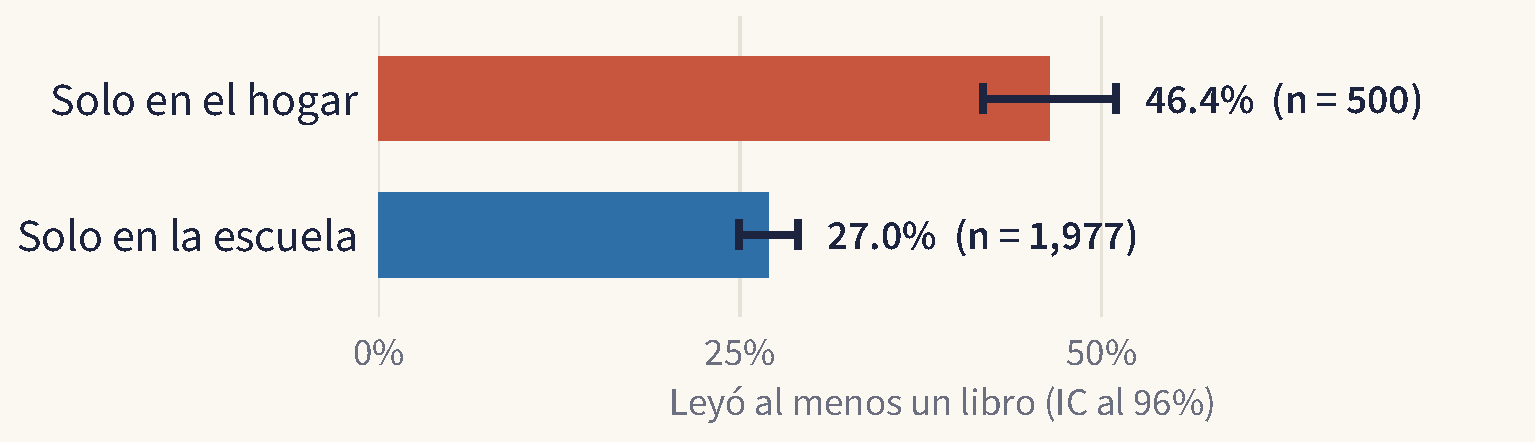
\includegraphics[width=18cm]{figs/f5_solo.pdf}};
  \node[anchor=north west, text width=17.4cm, align=left, font=\fontsize{20}{26}\selectfont, text=tinta] at ([xshift=1.6cm, yshift=-15.0cm]current page.north west)
    {Leyó al menos un libro el \textcolor{hogar}{\textbf{46.4\,\%}} del primer grupo y el \textcolor{escuela}{\textbf{27.0\,\%}} del segundo. Con 96\,\% de confianza, la diferencia es de \textbf{14 a 25 puntos} a favor de la casa (prueba z, \mbox{α = 0.04}).};
  % derecha
  \draw[crema, line width=3pt] ([xshift=20.4cm, yshift=-6.6cm]current page.north west) -- ++(0,-13.4);
  \node[anchor=north west, text width=17.4cm, align=left, font=\fontsize{20}{26}\selectfont, text=tinta] at ([xshift=21.4cm, yshift=-6.6cm]current page.north west)
    {¿Y si solo es que estudiaron más? \textbf{No}: dentro de cada nivel de escolaridad, tener mucho acceso en casa se asocia con \textbf{19 a 24 puntos más} de lectores.};
  \node[anchor=north west, inner sep=0] at ([xshift=21.0cm, yshift=-9.6cm]current page.north west) {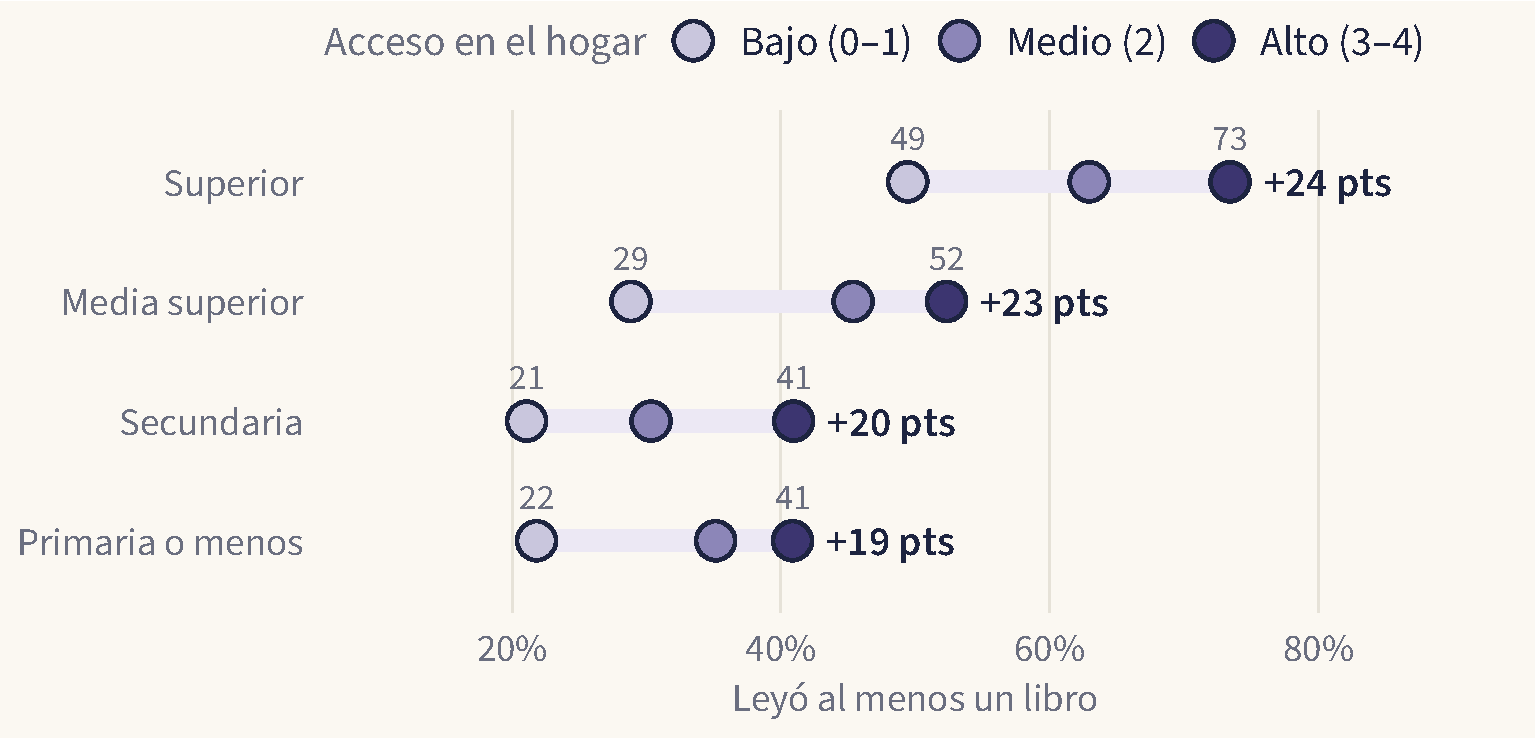
\includegraphics[width=18cm]{figs/f3_escolaridad.pdf}};
  \pie{gris}
\end{tikzpicture}
\newpage
% =============================================================== 3 · qué encontramos y qué proponemos
\pagecolor{papel}
\begin{tikzpicture}[remember picture, overlay]
  \paso{3}{gris}
  \node[anchor=north west, text=tinta, font=\serif\bfseries\fontsize{38}{44}\selectfont] at ([xshift=1.6cm, yshift=-2.4cm]current page.north west)
    {Qué encontramos y qué proponemos};
  \foreach \i/\num/\col/\txt in {
      0/{×\,2}/alto/{Con mucho acceso a la lectura en casa, la proporción de lectores es aproximadamente el doble (59.7\,\% contra 28.1\,\%).},
      1/{Casa}/hogar/{El hogar se asocia más que la escuela con leer, y el acceso en la escuela suele acompañar al que ya había en casa.},
      2/{< 1 libro}/escuela/{Entre quienes ya leen, la diferencia es de menos de un libro al año: el acceso pesa en \emph{volverse} lector.}} {
    \node[anchor=north west, fill=white, rounded corners=14pt, minimum width=11.9cm, minimum height=7.6cm] (c\i) at ({1.6+\i*12.6},-5.0) {};
    \node[anchor=north west, font=\serif\bfseries\fontsize{50}{56}\selectfont, text=\col] at ($(c\i.north west)+(0.8,-0.6)$) {\num};
    \node[anchor=north west, text width=10.4cm, align=left, font=\fontsize{19.5}{25}\selectfont, text=tinta] at ($(c\i.north west)+(0.8,-3.0)$) {\txt};
  }
  % propuesta
  \fill[tinta] ([yshift=-13.6cm]current page.north west) rectangle (current page.south east);
  \node[anchor=north west, text=oro, font=\sbf\fontsize{22}{26}\selectfont] at ([xshift=1.6cm, yshift=-14.4cm]current page.north west) {Propuesta: empezar por los niños con poco acceso en casa};
  \foreach \i/\t/\d in {0/1. Diagnosticar/{Medir en la escuela cuántos estímulos de lectura tiene cada niño en casa.},
                        1/2. Focalizar/{Priorizar a quienes tienen 0 o 1 estímulos.},
                        2/3. Llevar libros a casa/{Bibliotecas de aula y préstamo de libros para el hogar.},
                        3/4. Involucrar a las familias/{Talleres de lectura en voz alta para padres y cuidadores.}}
    \node[anchor=north west, text width=8.4cm, align=left, text=white, font=\fontsize{17.5}{22}\selectfont] at ({1.6+\i*9.4}, -16.0) {{\sbf\color{oro!80!white}\t}\\[4pt]\d};
  \node[anchor=south east, text=oro!70!white, font=\serif\itshape\fontsize{19}{23}\selectfont] at ([xshift=-1.6cm, yshift=2.0cm]current page.south east)
    {La desigualdad en el acceso empieza en casa… y ahí también puede empezar la solución.};
  \pie{white!55!tinta}
\end{tikzpicture}
\end{document}
